\section{Esercizio 11 -- Switch multistadio}
\subsection{Esercizio 11.1}
L'obiettivo è progettare e implementare in VHDL uno switch multistadio basato sul modello Omega Network. Consente di trasferire messaggi di 2 bit da un nodo sorgente a un nodo destinazione in una rete con 4 nodi. Il sistema deve implementare un meccanismo di instradamento deterministico, con un criterio di priorità fissa tra i nodi (il nodo 1 ha la priorità più alta, il nodo 4 la più bassa).

\begin{figure}[h]
    \centering
    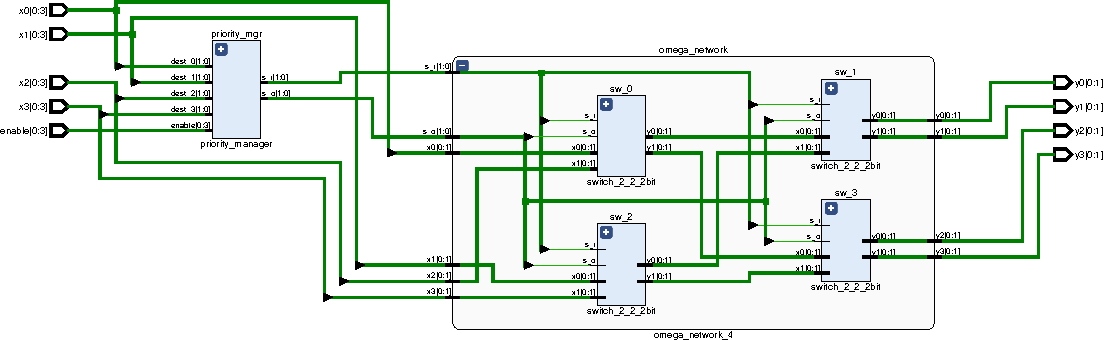
\includegraphics[width=\textwidth]{img/11_OMEGA_NETWORK.pdf}
    \caption{Schema a blocchi del sistema di comunicazione con switch multistadio}
    \label{fig:11_OMEGA_NETWORK}
\end{figure}

\subsubsection{Implementazione}

\begin{code}
    \inputminted{vhdl}{vhdl/omega_network_system.vhd}
    \caption{Implementazione del sistema di comunicazione con switch multistadio}
    \label{cod:omega_network_system}
\end{code}

\begin{code}
    \inputminted{vhdl}{vhdl/omega_network_4.vhd}
    \caption{Implementazione della rete Omega Network a 4 nodi}
    \label{cod:omega_network_4}
\end{code}

\begin{code}
    \inputminted{vhdl}{vhdl/switch_2_2_2bit.vhd}
    \caption{Implementazione dello switch 2:2 per pacchetti di 2 bit}
    \label{cod:switch_2_2_2bit}
\end{code}

\begin{code}
    \inputminted{vhdl}{vhdl/omega_network_priority_manager.vhd}
    \caption{Implementazione del gestore delle priorità}
    \label{cod:omega_network_priority_manager}
\end{code}

\paragraph{Funzionamento generale.}
L’Omega Network è un tipo di rete di interconnessione multistadio, utilizzata per il routing di pacchetti tra nodi sorgente e nodi destinazione:

\begin{itemize}
    \item È formata da più stadi di switch elementari (commutatori).
    \item Ogni stadio riorganizza i pacchetti seguendo uno schema predefinito.
    \item Può connettere N ingressi a N uscite usando $\log_{2}(N)$ stadi.
    \item Implementa un indirizzamento deterministico, basato sugli indirizzi della sorgente e della destinazione.
\end{itemize}

Nel caso specifico:

\begin{itemize}
    \item Vi sono 4 nodi sorgente e 4 nodi destinazione.
    \item Ogni pacchetto ha 2 bit di dati.
    \item La rete ha 2 stadi di switch ($\log_{2}(4) = 2$).
\end{itemize}

Il primo stadio collega gli ingressi (\texttt{x0}, \texttt{x1}, \texttt{x2}, \texttt{x3}) agli appositi ingressi del secondo stadio, seguendo il principio del \textit{perfect shuffling}. Il secondo stadio trasporta dunque i pacchetti alle uscite finali (\texttt{y0}, \texttt{y1}, \texttt{y2}, \texttt{y3}).

L'instradamento (routing) è regolato adi segnali di controllo \texttt{s\_i} ed \texttt{s\_o}, che sono la notazione binaria posizionale rispettivamente dell'indirizzo della sorgente e della destinazione. Ad ogni switch del livello \texttt{k} sono forniti i bit \texttt{s\_i[k]} e \texttt{s\_o[k]}:

\begin{itemize}
    \item Il bit \texttt{s\_i} decide l'indice della porta di ingresso da cui prelevare il pacchetto.
    \item Il bit \texttt{s\_o} decide l'indice della porta verso cui indirizzare il pacchetto.
\end{itemize}

Per la gestione dei conflitti viene adottato uno schema a priorità fissa: se due sorgenti vogliono inviare pacchetti alla stessa destinazione, viene scelta quella con la priorità più alta (ossia quella con indice minore). A tal proposito è presente il segnale \texttt{enable}: la sorgente manifesta la propria volontà di trasmettere un messaggio abilitando il bit di indice corrispondente al proprio indirizzo.

I messaggi sono di 4 bit: i 2 bit più significativi sono il contenuto del messaggio, i 2 bit meno significativi rappresentano l'indirizzo del nodo di destinazione.

I componenti principali del sistema sono:

\begin{enumerate}
    \item \texttt{omega\_network\_4}: un'architettura multistadio per instradare i pacchetti dai nodi sorgente ai nodi destinazione.
    \begin{itemize}
        \item Contiene 4 switch 2:2 controllati da segnali di selezione (\texttt{s\_i}, \texttt{s\_o}).
        \item Ingressi: 4 nodi sorgente (x0, x1, x2, x3) con 2 bit di dati ciascuno.
        \item Controllo: \texttt{s\_i} e \texttt{s\_o} gestiscono gli switch nei due stadi.
        \item Uscite: 4 nodi destinazione (y0, y1, y2, y3).
        \item Interconnessioni tra gli switch: vengono definiti i collegamenti interni tra il primo e il secondo stadio (\texttt{interconnection\_0\_1}, \texttt{interconnection\_0\_3}, \texttt{interconnection\_2\_1}, \texttt{interconnection\_2\_3}).
        \begin{itemize}
            \item Il primo switch collega \texttt{x0} e \texttt{x2} a due interconnessioni, attraverso la selezione di \texttt{s\_i(1)} e \texttt{s\_o(1)}.
            \item Il secondo switch collega le interconnessioni agli output \texttt{y0} e \texttt{y1}, attraverso la selezione di \texttt{s\_i(0)} e \texttt{s\_o(0)}.
            \item Il terzo switch collega \texttt{x1} e \texttt{x3} agli stadi intermedi, attraverso la selezione di \texttt{s\_i(1)} e \texttt{s\_o(1)}.
            \item Il quarto switch collega gli intermedi agli output finali \texttt{y2} e \texttt{y3}, attraverso la selezione di \texttt{s\_i(1)} e \texttt{s\_o(1)}.
        \end{itemize}
    \end{itemize}
    \item \texttt{switch\_2\_2\_2bit}: un commutatore 2:2 per pacchetti di 2 bit.
    \begin{itemize}
        \item Ha due segnali di controllo (\texttt{s\_i}, \texttt{s\_o}) per decidere il routing, due ingressi e due uscite.
    \end{itemize}
    \item \texttt{priority\_manager}: il gestore delle priorità.
    \begin{itemize}
        \item Determina i segnali di controllo (\texttt{s\_i}, \texttt{s\_o}) in base alla destinazione desiderata e alla priorità dei nodi.
        \item Estrae i bit di destinazione dai pacchetti in ingresso.
    \end{itemize}
    \item Segnali di ingresso/uscita:
    \begin{itemize}
        \item Ingresso: ogni nodo sorgente invia un messaggio di 4 bit.
        \begin{itemize}
            \item Primi 2 bit (dati): contenuto del pacchetto.
            \item Ultimi 2 bit (destinazione): indica il nodo destinatario.
        \end{itemize}
        \item Uscita: ogni nodo riceve un messaggio di 2 bit alla fine della trasmissione.
    \end{itemize}
\end{enumerate}

\paragraph{Struttura del codice.}
Il sistema è implementato con un approccio \texttt{structural} [Codice sorgente \ref{cod:omega_network_system}], in cui componenti più semplici vengono collegati tra loro per formare un sistema più complesso. I componenti principali sono:

\begin{enumerate}
    \item \texttt{omega\_network\_4} [Codice sorgente \ref{cod:omega_network_4}]: definisce la connessione tra ingressi e uscite della Omega Network.
    \begin{itemize}
        \item Prende in ingresso solo i primi 2 bit dei pacchetti di ogni nodo sorgente.
        \item Le uscite sono direttamente connesse ai nodi destinatari.
        \item I segnali \texttt{s\_i} e \texttt{s\_o} controllano gli switch interni della rete.
    \end{itemize}
    \item \texttt{switch\_2\_2\_2bit} [Codice sorgente \ref{cod:switch_2_2_2bit}]: implementa uno switch 2:2 per pacchetti di 2 bit.
    \begin{itemize}
        \item Prende in ingresso i bit \texttt{x\_0} e \texttt{x\_1}.
        \item Riceve i segnali di controllo \texttt{s\_i} e \texttt{s\_o} per decidere l'instradamento.
        \item Fornisce in uscita i segnali \texttt{y\_0} e \texttt{y\_1}.
        \item È implementato con un approccio strutturale, usando i componenti MUX 2:1 a 2 bit [Codice sorgente \ref{cod:mux_2_1_2bit}] e DMUX 1:2 a due bit [Codice sorgente \ref{cod:dmux_1_2_2bit}].
    \end{itemize}
    \item \texttt{priority\_manager} [Codice sorgente \ref{cod:omega_network_priority_manager}]: analizza quali nodi vogliono trasmettere e assegna i segnali di controllo \texttt{s\_i} e \texttt{s\_o}.
    \begin{itemize}
        \item Prende in ingresso i bit di destinazione per decidere l'instradamento.
        \item Genera i segnali di controllo \texttt{s\_i} e \texttt{s\_o} per la rete Omega.
        \item Gli ingressi \texttt{dest\_0}, \texttt{dest\_1}, \texttt{dest\_2}, \texttt{dest\_3} estraggono i bit di destinazione dai pacchetti in ingresso.
    \end{itemize}
\end{enumerate}

\subsubsection{Simulazione}
Per effettuare la simulazione il primo passo da compiere è la stesura del testbench. Prima di discuterne, è stato riportato il seguente codice:

\begin{code}
    \inputminted{vhdl}{vhdl/omega_network_tb.vhd}
    \caption{Testbench del sistema di comunicazione con switch multistadio}
    \label{cod:omega_network_tb}
\end{code}

Esso verifica il corretto funzionamento del sistema, che implementa una rete di interconnessione basata su un'Omega Network e un gestore di priorità. L'obiettivo principale è verificare il comportamento del sistema in diverse configurazioni di ingresso, assicurandosi che i pacchetti vengano instradati correttamente in base ai segnali di abilitazione (\texttt{enable}) e alle informazioni di destinazione contenute nei pacchetti.

La prima operazione svolta è stata la dichiarazione di un’entity. Si può notare che il corpo dell’entity è vuoto, poiché il testbench non rappresenta un componente hardware da implementare, ma serve esclusivamente per la simulazione e la verifica del corretto funzionamento del sistema.

\paragraph{Struttura del testbench.}
Il testbench è così strutturato:

\begin{enumerate}
    \item Dichiarazione del componente:
    \begin{itemize}
        \item \texttt{system}: il sistema di comunicazione con Omega Network e gestione della priorità.
    \end{itemize}
    \item Segnali e costanti:
    \begin{itemize}
        \item \texttt{x0}, \texttt{x1}, \texttt{x2}, \texttt{x3}: i messaggi dei nodi sorgente.
        \item \texttt{enable}: abilita i nodi per la trasmissione.
        \item \texttt{y0}, \texttt{y1}, \texttt{y2}, \texttt{y3}: catturano le uscite dal sistema per il test.
    \end{itemize}
    \item Processo di simulazione:
    \begin{itemize}
        \item \texttt{uut} (Unit Under Test).
        \begin{itemize}
            \item Rappresenta l'istanza del sistema collegata ai segnali di test.
            \item Gli ingressi \texttt{x0}, \texttt{x1}, \texttt{x2}, \texttt{x3} ed \texttt{enable} sono collegati ai segnali locali.
            \item Le uscite \texttt{y0}, \texttt{y1}, \texttt{y2}, \texttt{y3} riceveranno i dati dalla simulazione.
        \end{itemize}
        \item \texttt{stim\_proc}: il processo esegue la simulazione variando \texttt{enable} e controllando le uscite \texttt{y0}, \texttt{y1}, \texttt{y2}, \texttt{y3} (attendendo un certo tempo prima di cambiare i segnali).
    \end{itemize}
\end{enumerate}

\begin{figure}[h]
    \centering
    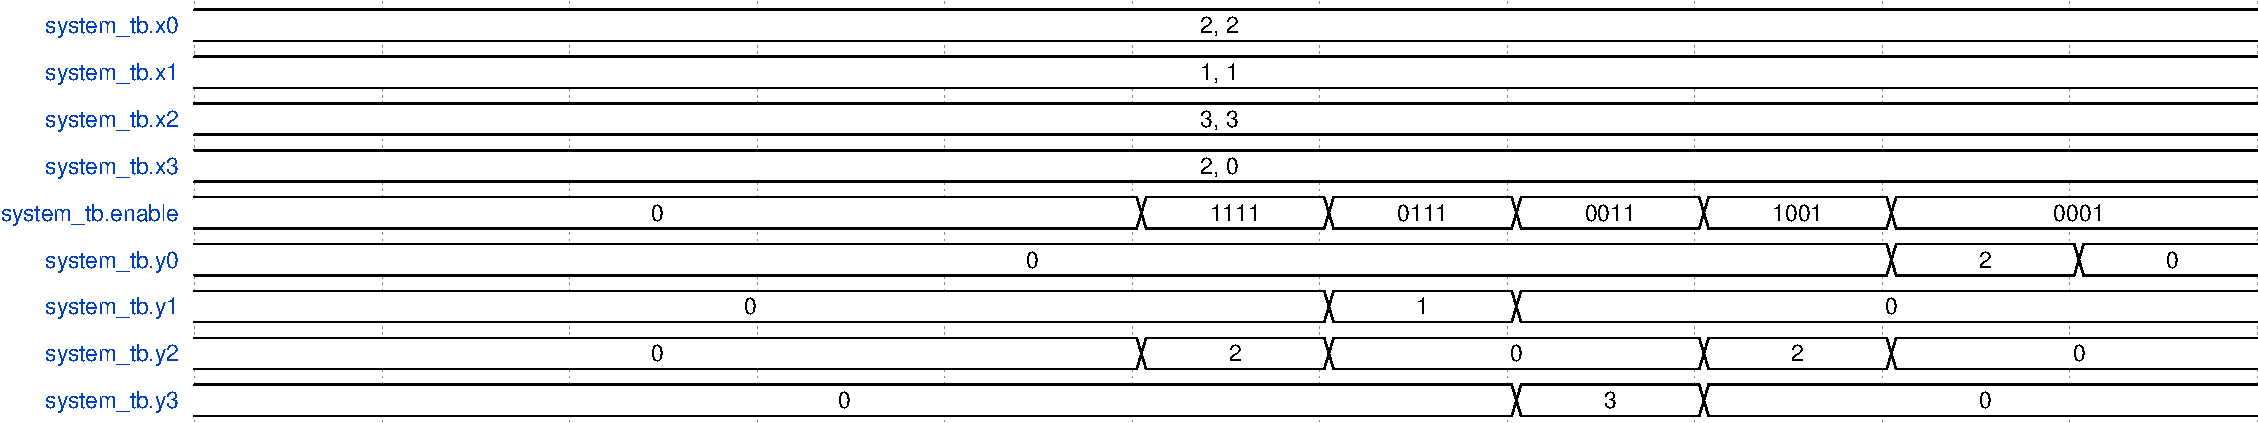
\includegraphics[width=\textwidth]{img/omega_network_tb.pdf}
    \caption{Simulazione del sistema di comunicazione con switch multistadio}
    \label{fig:omega_network_tb}
\end{figure}
